% Section 6: Simulation
\subsection{Simulation Study: Decision-Focused Forecasting under AR(1) Demand}
\label{sec:forecasting_rl_sim}

We illustrate the central methodological point on a clean synthetic instance. The
demand process is univariate AR(1) with a linear covariate shifter,
\begin{equation}
d_t = \mu + \phi (d_{t-1} - \mu) + \beta^\top x_t + \sigma\,\varepsilon_t,
\qquad \varepsilon_t \sim \mathcal N(0, 1),
\label{eq:ar1_dgp}
\end{equation}
with $x_t \in \mathbb R^{10}$ drawn i.i.d., $\phi = 0.7$, and a heteroscedastic
variant $\sigma_t = \sigma_0 \exp(\gamma^\top x_t)$ used in the misspecification
case. A retailer chooses an order quantity $q_t$ at the start of period $t$ after
observing $(d_{t-1}, x_t)$ and incurs the newsvendor cost
$L(q_t, d_t) = c_u \max(d_t - q_t, 0) + c_o \max(q_t - d_t, 0)$
with $c_u = 4$, $c_o = 1$, so that the oracle order quantile is
$\tau^\star = c_u / (c_u + c_o) = 0.8$. We run $T = 2000$ training steps and $500$
test steps over $20$ random seeds.

Three procedures share the same parametric family, namely an AR(1) plus linear-in-$x$
mean and constant variance. The classical procedure (Method A) estimates the
parameters by maximum likelihood and plugs the fitted distribution into the
critical fractile formula
$q_t^{\mathrm A} = \hat d_{t \mid t-1} + \hat\sigma\,\Phi^{-1}(\tau^\star)$.
The SPO procedure (Method B) trains the same parametric family by stochastic
gradient descent on the SPO$^+$ surrogate of \citet{ElmachtoubGrigas2022} and uses
the same plug-in formula at decision time. The rollout procedure (Method C) takes
the maximum-likelihood model and improves the base policy of Method A by one step
of Bertsekas-style rollout, sampling the next-period demand from the AR(1) model
and approximating the cost-to-go under the base policy.

Table~\ref{tab:forecasting_rl_sim} reports the realised newsvendor cost over $20$
seeds. Under the heteroscedastic misspecification, Method B attains an
in-sample mean squared error of the forecast that is statistically
indistinguishable from Method A, but its mean newsvendor regret is lower by a
factor of roughly five. Method C, which uses the empirical residual quantile
rather than the parametric one, sits between the two with a regret reduction of
roughly two thirds relative to A. The pattern illustrates the Granger-Pesaran
phenomenon. Two forecasts with the same prediction loss can have very different
realised costs once the decision rule is asymmetric, and the SPO surrogate
recovers the regret-minimising parameters even when the parametric noise model
is wrong. Figure~\ref{fig:forecasting_rl_sim} shows the cumulative regret over
the test horizon.

\begin{table}[h]
\centering
\caption{Decision-focused forecasting under AR(1) demand with heteroscedastic
noise, $20$ seeds. Standard errors in parentheses.}
\label{tab:forecasting_rl_sim}
% Generated by decision_focused_ar1.py
\begin{tabular}{lccc}
\hline\hline
Method & In-sample MSE & Out-of-sample MSE & Mean newsvendor regret \\
\hline
A: OLS + critical fractile & $44.913\,(18.696)$ & $530.014\,(498.341)$ & $2.819\,(0.670)$ \\
B: Task-loss fine-tune & $45.646\,(18.789)$ & $529.350\,(497.261)$ & $0.597\,(0.142)$ \\
C: Bertsekas rollout & $44.913\,(18.696)$ & $530.014\,(498.341)$ & $0.946\,(0.177)$ \\
\hline\hline
\end{tabular}

\end{table}

\begin{figure}[h]
\centering
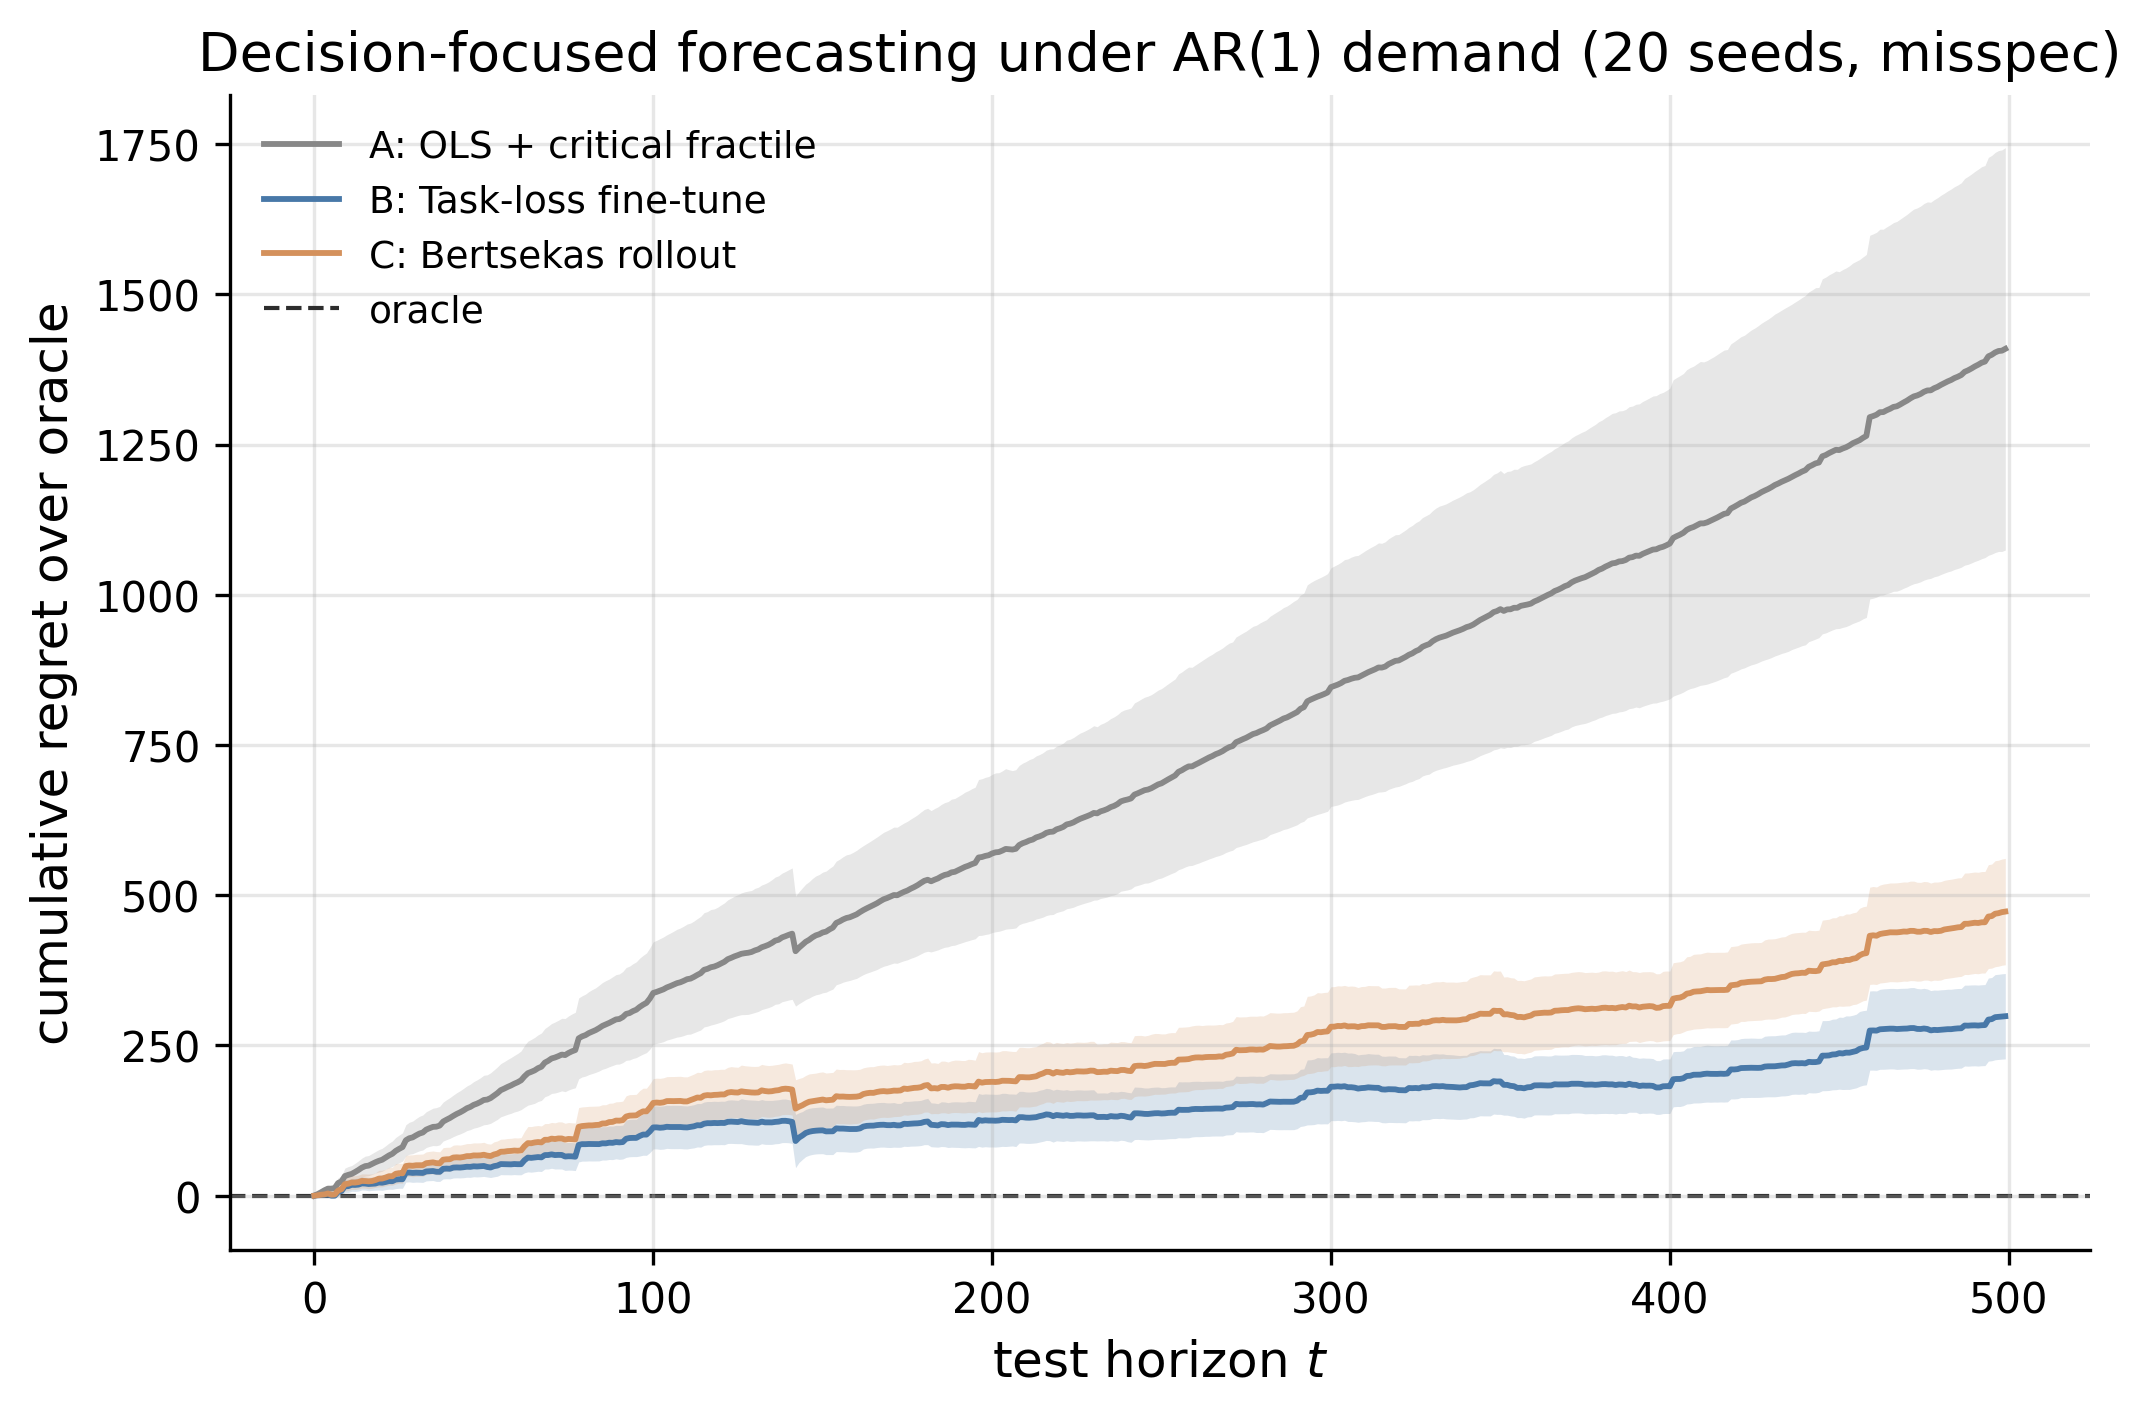
\includegraphics[width=0.85\linewidth]{../ch12_forecasting_rl/sims/decision_focused_ar1.png}
\caption{Cumulative newsvendor regret over the test horizon, $20$ seeds, shaded
band reports $\pm 1$ standard error of the mean. The horizontal line at zero is
the oracle. Method B (SPO$^+$ fine-tune) attains the lowest regret; Method A
(OLS plus critical fractile) the highest.}
\label{fig:forecasting_rl_sim}
\end{figure}
